
%(BEGIN_QUESTION)
% Copyright 2011, Tony R. Kuphaldt, released under the Creative Commons Attribution License (v 1.0)
% This means you may do almost anything with this work of mine, so long as you give me proper credit

Et regnearkprogram kan brukes som simulator for en {\it median select}-funksjon, der medianen av tre innverdier velges.

Start med å lage et eget regneark etter formatet vist under, slik at hvem som helst kan skrive inn tre verdier i celler på venstre side av arket, mens regnearket velger og viser medianverdien i en celle mot høyre side. Gul (inngang) og blå (utgang) cellefarge er valgfritt:

$$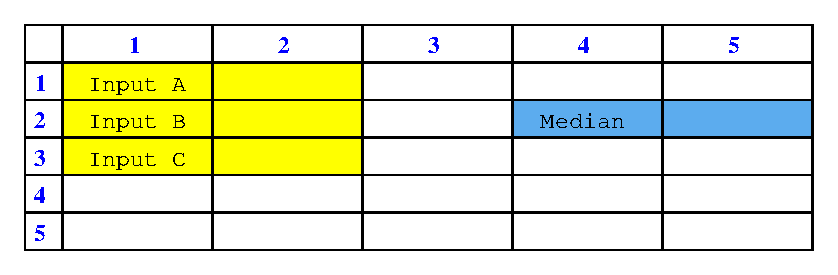
\includegraphics[width=15.5cm]{i00790x01.eps}$$

Hvor kan en median-select-funksjon brukes i et prosessreguleringssystem?

\vskip 20pt \vbox{\hrule \hbox{\strut \vrule{} {\bf Forslag til sokratisk diskusjon} \vrule} \hrule}

\begin{itemize}
\item{} Det finnes definitivt mer enn én måte å implementere denne funksjonen i et regnearkprogram. Identifiser minst to av dem.
\end{itemize}

\underbar{file i00790}
%(END_QUESTION)





%(BEGIN_ANSWER)


%(END_ANSWER)





%(BEGIN_NOTES)


%INDEX% Regnearkøvelse: median-select-funksjon
%INDEX% Relé, beregningsfunksjon: median select

%(END_NOTES)


